\documentclass[border=10pt]{standalone}

\usepackage{tikz}
\usepackage{tikzsymbols}
\usetikzlibrary{calc,patterns,shapes.geometric}

\def\centerarc[#1](#2)(#3:#4:#5){\draw[#1] ($(#2)+({#5*cos(#3)},{#5*sin(#3)})$) arc (#3:#4:#5);}

\begin{document}
	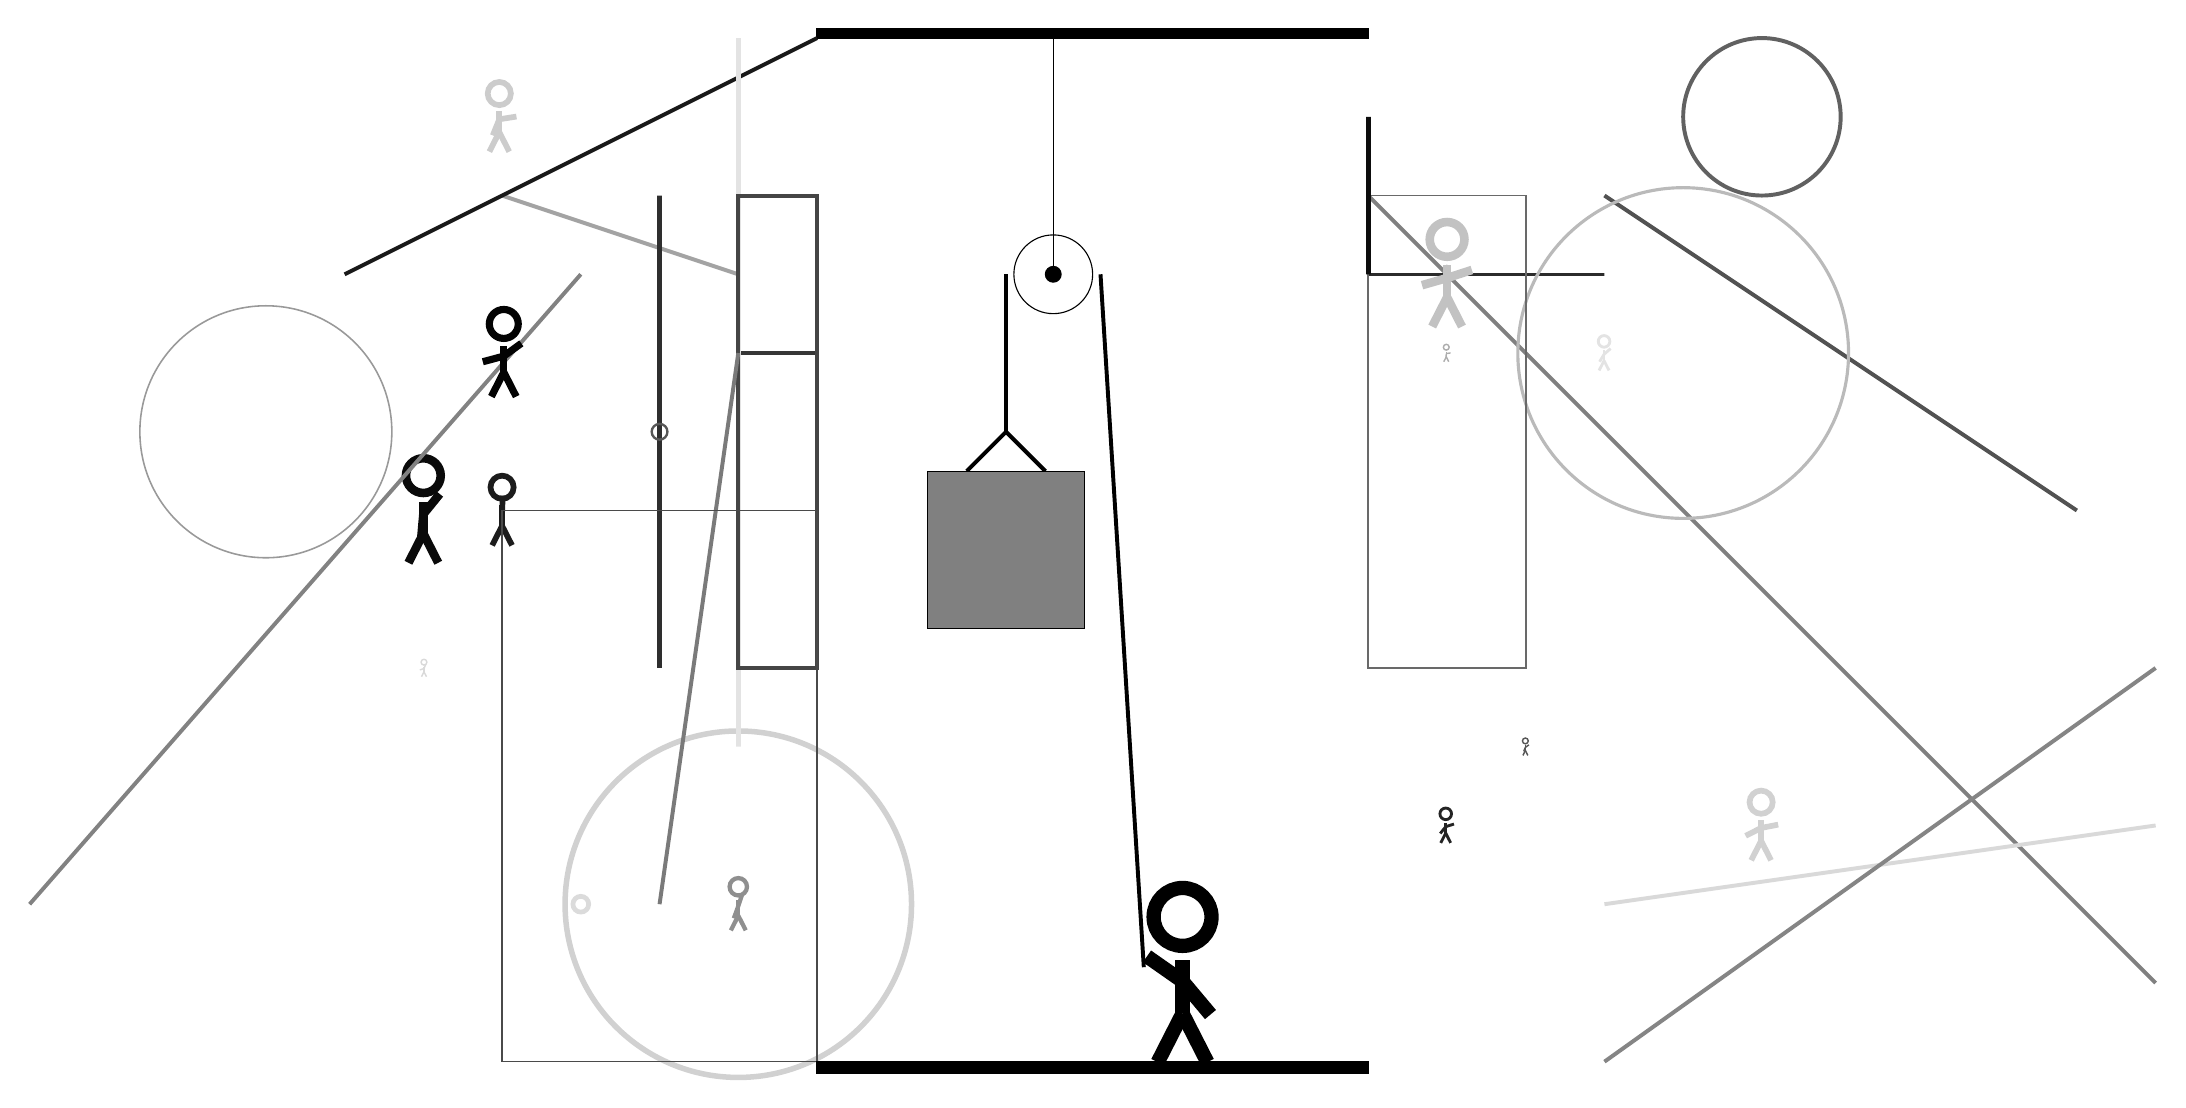
\begin{tikzpicture}
		%%%%% START %%%%%
		
		\draw[fill=black] (-2, 10) rectangle (5, 10.125);
		
		\draw (1, 7) circle (0.5);
		\draw[fill=black] (1, 7) circle (0.1);
		\draw (1, 10) -- (1, 7);
		
		\draw [line width=0.2mm, color=black!40](-9, 5) circle (1.6);
		
		\draw[line width=0.5mm, color=black!36](-6, 8) -- (-3, 7);
		\draw[line width=0.5mm, color=black!50](5, 8) -- (15, -2);
		\draw[line width=0.5mm, color=black!90](-2, 10) -- (-8, 7);
		
		\draw[line width=0.5mm, color=black!68](8, 8) -- (14, 4);
		\draw [line width=0.5mm, color=black!62](10, 9) circle (1.0);
		
		\node[line width=0.7mm, color=black!15] at (-7, 2) {\Strichmaxerl[1][17][67]};
		\draw[line width=0.7mm, color=black!82] (-4, 2) rectangle (-4, 8);
		\node[line width=0.7mm, color=black!11] at (8, 6) {\Strichmaxerl[2][59][41]};
		
		\draw [line width=0.6mm, color=black!14](-5, -1) circle (0.1);
		
		\draw [line width=0.7mm, color=black!18](-3, -1) circle (2.2);
		
		\node[line width=0.6mm, color=black!96] at (-7, 4) {\Strichmaxerl[6][85][51]};
		\draw[line width=0.5mm, color=black!79] (-2, 2) rectangle (-3, 6);
		
		\draw[line width=0.4mm, color=black!83] (5, 7) rectangle (8, 7);
		\node[line width=0.4mm, color=black!93] at (6, 7) {\Strichmaxerl[1][50][60]};
		\draw[line width=0.5mm, color=black!49](-5, 7) -- (-12, -1);
		
		\draw[line width=0.5mm, color=black!15](8, -1) -- (15, 0);
		\draw [line width=0.3mm, color=black!66](-4, 5) circle (0.1);
		\draw [line width=0.4mm, color=black!27](9, 6) circle (2.1);
		\node[line width=0.2mm, color=black!44] at (-3, -1) {\Strichmaxerl[3][70][72]};
		\node[line width=0.6mm, color=black!24] at (6, 7) {\Strichmaxerl[6][16][18]};
		
		\draw[line width=0.6mm, color=black!11] (-3, 1) rectangle (-3, 10);
		\draw[line width=0.5mm, color=black!48](8, -3) -- (15, 2);
		\node[line width=0.7mm, color=black!99] at (-6, 6) {\Strichmaxerl[5][15][36]};
		\draw[line width=0.2mm, color=black!59] (5, 2) rectangle (7, 8);
		
		\node[line width=0.7mm, color=black!20] at (-6, 9) {\Strichmaxerl[4][68][9]};
		\draw[line width=0.5mm, color=black!73] (-2, 8) rectangle (-3, 2);
		\node[line width=0.3mm, color=black!89] at (-6, 4) {\Strichmaxerl[4][90][88]};
		
		\node[line width=0.2mm, color=black!18] at (10, 0) {\Strichmaxerl[4][27][11]};
		
		\node[line width=0.4mm, color=black!86] at (6, 0) {\Strichmaxerl[2][51][18]};
		\draw[line width=0.5mm, color=black!52](-3, 6) -- (-4, -1);
		\node[line width=0.5mm, color=black!66] at (7, 1) {\Strichmaxerl[1][67][35]};
		\node[line width=0.4mm, color=black!32] at (6, 6) {\Strichmaxerl[1][87][10]};
		
		\draw[line width=0.6mm, color=black!95] (5, 7) rectangle (5, 9);
		\draw[line width=0.2mm, color=black!71] (-2, -3) rectangle (-6, 4);
		
		\draw[line width=0.5mm] (-0.1, 4.5) -- (0.4, 5.0) -- (0.9, 4.5);
		\draw[fill=black!50] (-0.6, 4.5) rectangle (1.4, 2.5);
		
		\draw[line width=0.5mm] (0.4, 7) -- (0.4, 5.0);
		\centerarc[line width=0.5mm](1, 7)(0:180:0.6);
		\draw[line width=0.5mm](1.6, 7) -- (2.15, -1.8);
		
		\node at (2.6, -1.9) {\Strichmaxerl[10][-35][-50]};
		
		\draw[fill=black] (-2, -3) rectangle (5, -3.15);
		
		%%%%% END %%%%%
	\end{tikzpicture}
\end{document}